\documentclass{article}

\usepackage{array}
\usepackage{etoolbox}
\usepackage{fancyhdr}
\usepackage{geometry} 
\usepackage{graphicx}
\usepackage{soul}
\usepackage{titling}
\usepackage{url}

%%%%%%%%%%%%%%%%%%%%%%%%%%%%%%%%%%%%%%%%%%%%%%%%%%%%%%%%%%%%
% BEGIN METADATA: Edit the following as appropriate
%%%%%%%%%%%%%%%%%%%%%%%%%%%%%%%%%%%%%%%%%%%%%%%%%%%%%%%%%%%%

\title{Real-Time Safety Monitoring System for Industrial Workplaces Using AI and Computer Vision}  % the title of your project
\newcommand\shorttitle{\thetitle}  % if needed: a shorter title for the document header
% Team members.
\newcommand\secondname{Asad Ullah Chaudhry} % full name
\newcommand\secondid{ac07408}        % ID, e.g. xy01234
\newcommand\thirdname{Muhammad Arsalan Hussain}  % full name
\newcommand\thirdid{mh07607}         % ID, e.g. xy01234
\newcommand\fourthname{Muzzammil Kamran Sattar}  % full name
\newcommand\fourthid{ms07164}  
\newcommand\firstname{Syed Ahad Ali}  % full name
\newcommand\firstid{sa07753}         % ID, e.g. xy01234

\newenvironment{tight_enumerate}{
\begin{enumerate}
  \setlength{\itemsep}{0pt}
  \setlength{\parskip}{0pt}
}{\end{enumerate}}


%%%%%%%%%%%%%%%%%%%%%%%%%%%%%%%%%%%%%%%%%%%%%%%%%%%%%%%%%%%%
% END METADATA: Do not edit the preamble any further.
%%%%%%%%%%%%%%%%%%%%%%%%%%%%%%%%%%%%%%%%%%%%%%%%%%%%%%%%%%%%

\pagestyle{fancy}
\lhead{Kaavish Proposal}
\rhead{Fall 2024}
\cfoot{Page \thepage}
\renewcommand{\footrulewidth}{0.4pt}

\newcommand\instruction[1]{\textit{#1}}

\begin{document}

% Cover page.
\begin{titlepage}

\center % Center everything on the page
 
%----------------------------------------------------------------------------------------
%	HEADING SECTIONS
%----------------------------------------------------------------------------------------

\textsc{
  {\LARGE \bf \thetitle}\\\bigskip\bigskip % Your Project Title
  {\large
    Kaavish Project Proposal\\\bigskip
    By}
}\\\bigskip 

%----------------------------------------------------------------------------------------
%	AUTHOR SECTION
%----------------------------------------------------------------------------------------

{\large
  \begin{tabular}{ll}
    \firstname & (\firstid@st.habib.edu.pk) \\
    \secondname & (\secondid@st.habib.edu.pk) \\
    \thirdname & (\thirdid@st.habib.edu.pk) \\
    \ifdef{\fourthname}{\fourthname & (\fourthid@st.habib.edu.pk) \\}{}
    \ifdef{\fifthname}{\fifthname & (\fifthid@st.habib.edu.pk) \\}{}
  \end{tabular}
}
\bigskip\bigskip\bigskip

{\large \today}\\\bigskip\bigskip

\includegraphics[height=5cm]{HU_logo}\\\bigskip
 
%----------------------------------------------------------------------------------------
{\large
  In partial fulfillment of the requirement for \\\medskip
Bachelor of Science \\\medskip
Computer Science
}\\\bigskip\bigskip\bigskip

{\large
  \textsc{
    Dhanani School of Science and Engineering\\\bigskip
    Habib University\\\bigskip 
    Fall 2024
  }\\\bigskip\bigskip 
  Copyright @ 2024 Habib University
}

\end{titlepage}


%%%%%%%%%%%%%%%%%%%%%%%%%%%%%%%%%%%%%%%%%%%%%%%%%%%%%%%%%%%%
% DATA: Populate the rest of the document as instructed.
%%%%%%%%%%%%%%%%%%%%%%%%%%%%%%%%%%%%%%%%%%%%%%%%%%%%%%%%%%%%
\section{Abstract}
Pakistan's industrial sector, employing millions in manufacturing and construction, faces significant safety challenges, with 1.9 million workers reporting injuries in 2020-2021 alone.
These incidents often result in severe financial strain for low-wage workers, particularly in a country with limited labor regulations and safety oversight. 
This project aims to improve workplace safety by developing a real-time monitoring system utilizing computer vision and deep learning for Dawlence's sheet metal plant in Karachi. 
The system will analyze video footage from factory CCTV cameras to detect unsafe behaviors, such as failure to wear protective gear or operating machinery unsafely in real-time.  
By providing real-time alerts, this system will help prevent accidents, ensuring both employee safety and operational compliance for Dawlence. 
It will also provide statistics and insights to help improve Dawlance's safety protocols and reduce the risk of accidents.  
With a scalable design, the system can be adapted to various industrial settings, making it a valuable tool for reducing workplace injuries and promoting a safer working environment.


\section{Problem definition}

Pakistan has an employed population of 71.76 million \cite{governmentofpakistan2021PakistanLabourForce2021} with a significant portion of the workforce
employed in the manufacturing (14.9\%) and construction (14.4\%) sectors \cite{governmentofpakistan2021PakistanLabourForce2021}. 
Out of the total workforce population, 1.9 million (2.7\% of total) people faced a work related injury in 2020-2021. Of these injured people,
40.5\% of workers had to consult a medical professional, 11.7\% had to get hospitalized and 31.6\% were forced to take took time off work becuase of their injury
\cite{governmentofpakistan2021PakistanLabourForce2021}. The labour workforce in the industrial sector (engaged in assembly and manufacturing) is one of the most dangerous 
sectors to work in, accounting for 20\% of all workplace injuries in 2020-2021 \cite{governmentofpakistan2021PakistanLabourForce2021}.
With the monthly average income in the manufacturing sector being 22,000 PKR \cite{governmentofpakistan2021PakistanLabourForce2021}, 
such injuries can have a significant impact on the financial stability of the workers and their families with many not being able to afford healthcare services at all. 
% Formal sector employers usually hestitate to provide insurance for their workers, and the government does not have a comprehensive social security system in place to support these injured workers.
% The informal sector workers are left to fend for themselves, as informal sector jobs don't involve formal work agreements and thus are deprived of their labour rights entirely. The data on the number of injuries 
% or deaths that occur in the informal sector can also be inaccurate due to it's unregulated nature. 
Pakistan stands as one of the countries with the least amount of regulation and protection when it comes to labor rights. For a labor force of 10.63 million (that is part of the formal sector),
Pakistan has nearly 517 labour inspectors which means one inspector for more than 20,560 workers\cite{Whistlers} highlighting the neglect of Labour rights, safety protocols and education of the workers into safe practices.
\\ \\
This project aims to address the issue of workplace safety in the industrial sector by developing a real-time safety monitoring system that can detect unsafe behaviors and conditions in the workplace. 
Such a system can help prevent accidents and injuries by alerting workers and supervisors when unsafe conditions are detected, allowing them to take corrective action \textbf{before} an accident occurs.
The system will use computer vision and deep learning techniques to analyze video footage from CCTV cameras installed in the factory and identify safety hazards in real time.

%add some space
\vspace{3.5cm}
Our system goals include the following:
\begin{itemize}
    \item Ensuring safety equipment is being worn, including gloves and hard tipped shoes
    \item Ensuring workers aren't accessing barricaded equipment when it's operational. 
    \item Ensuring the plant pathway (denoted by yellow lines on the floor) remains obstacle free
    \item Ensuring forklift operators are practicing safe usage
    \item Ensuring prompt response if a worker falls
    \item Ensuring correct and safe usage of the hydraulic presses by the workers
\end{itemize}
Through notifications and alerts, the system will provide real-time feedback to workers and supervisors, enabling them to take immediate action to prevent accidents and injuries
The system will also identify trends and patterns in workplace safety through saving incident data and generating reports based on that data. These reports can then allow Dawlance to take proactive measures to improve safety protocols and reduce the risk of accidents.
Finally, the system will be designed to be scalable and adaptable to different types of industrial environments, making it suitable for a wide range of applications in the manufacturing and construction sectors.

\begin{figure}[h]
    
    \centering
    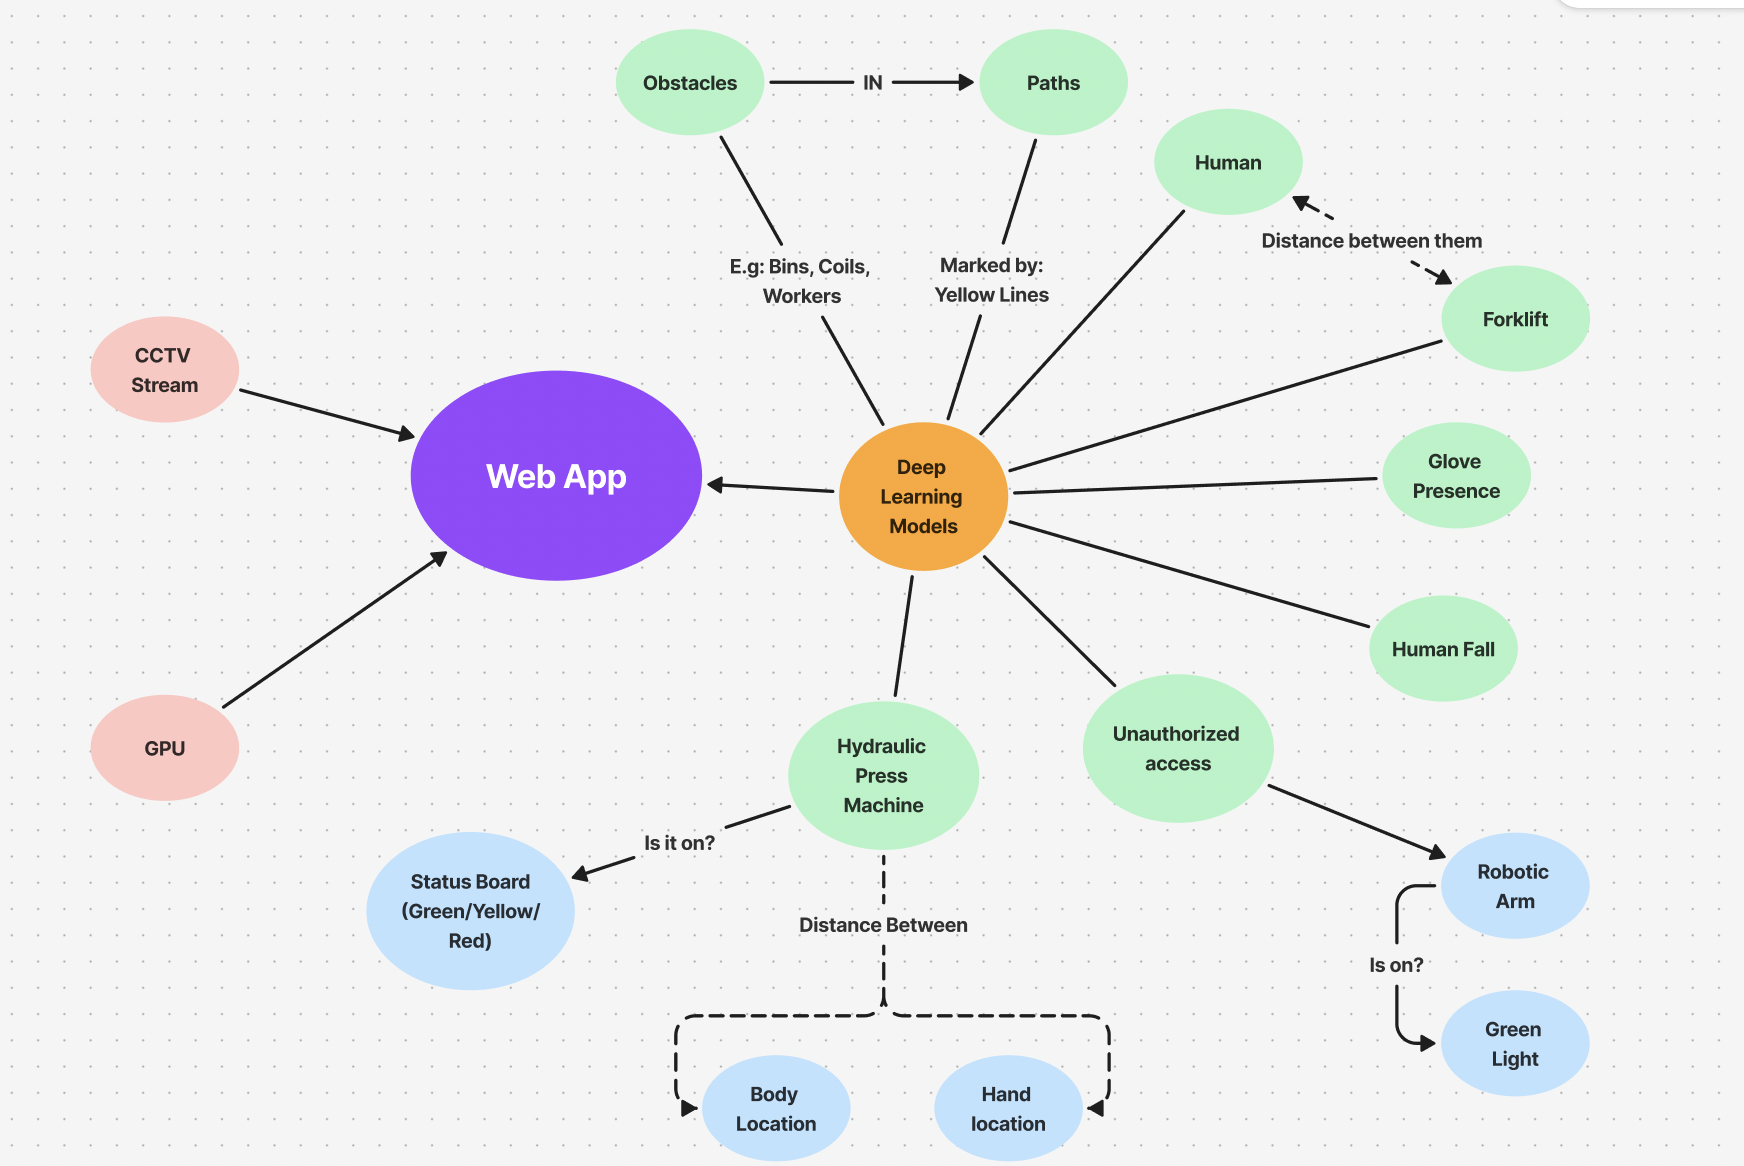
\includegraphics[height = 9cm]{overview.png}
    \caption{High Level Overview of the System}
\end{figure}

\section{Social relevance}

For \textbf{workers}, in Pakistan, the system offers a means of improving personal safety on the job and 
avoid the financial burden assosicated with injury. Many industrial workers earn relatively low wages and lack comprehensive insurance coverage, the financial impact of a workplace injury 
can be devastating. This system protects workers from such life-altering events by altering on-site staff that an intervention may be needed.
\\ \\
By continuously monitoring unsafe conditions and behaviors and providing analytics, our system will enable \textbf{Manufactures} to take both reactive actions and preemptive actions to prevent accidents, hence ensuring compliance with safety regulations.
This minimizes the financial risks and legal consequences associated with workplace injuries. As per our industry visit, Dawlence is committed to worker safety and has a lot of protections already in place. 
This system would be the last line of defense in their arsenal, to stand true to their motto of `An employee shouldn't be able to hurt themself even if they deliberately try`'. 
\\ \\
Given the shortage of labor inspector,this automated system can significantly reduce the reliance on manual inspections. 
Furthermore, it can even render the inspector system obsolete. With the government ill-equipped to handle the large number of workers in the country, scaling this system across different industries could provide a much-needed solution to ensure worker safety nationwide.

% \\ \\
% Such automation can help supliment periodic manual inspections by 24/7 safety monitoring, and it's scalibility means it can be applied to multiple 
% plants and factories with small changes. This approach not only promotes a safer work environment but also encourages a cultural shift towards prioritizing worker safety in Pakistan's industrial sector.


\section{Originality/Novelty}
% \instruction{Describe the value of solving the problem. Compare and contrast with any existing solutions.}
\subsection{Value of Solving the Problem}

Currently, companies in the manufacturing sector, such as Dawlence, implement a wide range of safety standards. These standards include, but are not limited to, the prevention of unsafe machine operation through the use of light sensors, safety protocols, and barricading heavy and sensitive moving equipment such as large actuators and robotic arms.
\\
Our system provides an additional layer on top of the existing safety measures. While several of the above systems and protocols are in place, there is always a possibility that they may fail. Dawlence's vision is that if these systems and measures do fail, an on-site overseer should be notified so that last-minute human intervention can take place.
\\
Furthermore, there is currently no system in place that, for example, detects the presence of obstacles in the path of moving machinery or identifies the presence of an individual in an unauthorized area after they've entered. The current system involves manual checks through a single security CCTV camera or through an on-site overseer, which is highly inefficient and resource- and time-consuming. Our system simplifies this process through real-time automation and detection, providing on-site overseers with simple and effective alerts, notifying them when and where a safety hazard is present. 

\subsection{Comparison with Existing Solutions}
Existing solutions for workplace safety monitoring are often manual, periodic, and reliant on human inspectors which is a kind of reactive approach rather than a proactive one. These solutions are limited in their effectiveness, as they cannot provide real-time feedback or continuous monitoring of workplace conditions. Apart from that, as witnessed in our visit to their sheet metal manufacturing plant, the dawlance team has automated many of the safety protocols already, such as ultrasonic sensors to detect if a worker is exposed to danger in a machine while the machine is being operated, this makes the machine stop immediately. However, according to the dawlance team, the system is not foolproof and can be bypassed by the workers. This is where our system comes in, it will be able to detect if a worker is not wearing the required safety equipment and will be able to alert the worker and the supervisor in real-time, thus preventing any accidents from happening.

\section{CS contribution}
This project draws heavily on advanced concepts from computer science and intermediate concepts from computer engineering. It demonstrably incorporates elements from deep learning, computer vision, data communication, integrated systems and software engineering as follows:

\begin{enumerate}
    \item \textbf{Introduction to Deep Learning}: The heart of the project is fine-tuning AI models to make them capable of identifying safety hazards in real time through image and video data. The core concepts from deep learning, including Convolutional Neural Networks (CNNs), object detection, and transfer learning, will be used to create a highly accurate detection system. This component's main code will be leveraging frameworks such as TensorFlow, PyTorch and Ultralytics for fine-tuning and inference.
    However, the biggest challenge is ,of course, data preparation. It mainly includes cleaning video footage, annotating safety-relevant scenes (e.g., workers without protective gear, machines) and safety irrelevant scenes. These tasks will ensure that the AI models have relevant high quality data to work with. This is the most straightforward part of the project but also the most laborious.
    \item \textbf{Computer Vision}: The AI models' functionality revolves around recognizing and classifying images, including detecting protective equipment (like gloves and vests), state of machines (like ON or OFF) and identifying hazardous zones. The project will employ techniques such as image segmentation, object detection and classification, distance calculation etc. Furthermore, OpenCV, Ultralytics and other image processing libraries will be used to extract and pre-process visual data captured by CCTV cameras.    
    \item \textbf{Embedded Systems}: The project integrates with CCTV camera systems, and part of the implementation may involve working with embedded systems to ensure efficient data capture. For example, cameras may be required to follow a variable motion routine (FSM), zoom in via lens and focus on a workplace hazard or incident. This component's requirement is inversely proportional to the number of cameras that Dawlance installs in their warehouses for this project.        
    \item \textbf{Web Development}: The project will involve developing a user-friendly web-based dashboard to display real-time data and analytics regarding workplace safety compliance. This web app will allow users to monitor safety alerts and trends.
    \item \textbf{Software Engineering}: The overall architecture of the project will follow best practices in software engineering, including modular design, agile development, continuous integration, and deployment (CI/CD). Due to the large scope of the project, it would be best to deliver modest features in multiple sprints starting with easier functionality like PPE detection.
\end{enumerate}

\section{Scope and Deliverables}
The scope of this project is designed to align with the expertise of the team and the year-long timeline. It encompasses various interdisciplinary tasks that will be discussed after the scope is justified:
\begin{enumerate}
    \item \textbf{Dataset creation from scratch}: The critical part of this project will be the creation and preparation of a custom dataset that includes annotated video footage of industrial environments. This dataset will be used for training and fine-tuning deep learning models. The dataset will include safety-relevant scenes (e.g., workers not wearing protective gear) and irrelevant scenes to ensure high-quality training data for the AI models. This step, though straightforward, will be labor-intensive as not only will good annotation of data be required but careful designing of minimum amount of scenes (i.e. video clips) whilst ensuring enough diversity in data to represent various safety hazards. All four team members will have to be effective, efficient and quick in their annotations/creations.
    \item \textbf{Integration of various technologies}: The project requires the integration of several technologies, including deep learning, computer vision, real-time data communication, cloud computing, and embedded systems. Each of these components must seamlessly work together to detect safety hazards and trigger appropriate actions, such as sending alerts or adjusting camera focus. The system must also ensure very low latency in real time detection. The scope of this integration is well-suited to a year-long project, where each phase will be tackled in sprints.
    \item \textbf{Interdiscplinary Nature}: As written in the previous section, this project involves software development, deep learning, computer vision, hardware setup (camera systems), and safety protocol knowledge. The interdisciplinary nature underscores the need for expertise across domains, such as AI model fine-tuning, computer networking for real-time data transmission, and embedded systems for camera control. The scope justifies a year-long duration, as it requires collaboration across multiple fields to ensure the system not only detects hazards but operates efficiently within a real-world industrial setting. This complexity allows each team member to contribute their specialized skills.
\end{enumerate}

\subsection{Foreseeable Deliverables}
\begin{enumerate}
    \item \textbf{S.R.S Document}: A comprehensive document outlining all the functional and non-functional requirements, serving as the foundation for the project's development. 
    \item \textbf{Deployed dashboard web application}: A web-based dashboard that allows monitoring of safety compliance in real time. This application will feature widget(s) for data-driven insights, enabling safety officers to track incidents, visualize trends, and find the gaps in current safety measures taken. The dashboard will also be integrated with our hazard detection system, allowing safety officers to view detected hazards and their status.
    % this will contain a widget for data driven insights
    \item \textbf{Notification system}: A multi-channel notification system that triggers alerts when safety violations are detected. This system could include a range of alert types, such as web app notifications, email alerts, voice alarms, or even SMS notifications. It will ensure that safety concerns are flagged immediately, so that there is rapid intervention in hazardous situations.
    % might include an alarm system, voice alert, web app notifications, email
    \item \textbf{The hazard detection AI model}: The core deliverable of the project, this AI model will be capable of identifying safety violations in real-time video footage. It will be fine-tuned to detect personal protective equipment (PPE), hazardous zones, and machine states. The model will be integrated into the larger system for seamless operation with real-time data from CCTV cameras.
    \item \textbf{Post processing algorithm}: This algorithm will, of course, handle logic after the AI model detects objects or hazards. It will determine if the detected situation meets predefined safety requirements. If violations are found, appropriate actions will be triggered for each hazard, such as sending alerts or activating a voice alarm. However, it may also contain a component to be used for further detection; it is possible that image processing or traditional CV techniques will be required after a pass through YOLOV8 for distance calculation, relevancy of hazard (e.g. worker may be too close to machinery which would typically be a hazard but it may not be considered one if the machine's state is OFF) etc.
    % this will include logic to check if the requirements are met based on the objects detected from AI model. If not, required action will be taken i.e. email notification, voice alarm etc.
    \item \textbf{Documentation}: Full technical documentation covering all aspects of the system's development, including setup instructions, user guides, and maintenance procedures. 
\end{enumerate}

\section{Feasibility}

\subsection{Datasets}
\begin{enumerate}
    \item \textbf{Datasets}: We will be using data from Dawlence's CCTV cameras to test and train our models. We will also be creating our own dataset to fine-tune the model. We will also use publicly available datasets for training and testing purposes.
    \item \textbf{Data Annotation}: The data will be annotated by the team members themselves. This will be a laborious task but will ensure that the data is annotated correctly and is of high quality.
    \item \textbf{Computer Resources and Hardware}
        \begin{enumerate}
        \item GPU computing power to fine-tune the computer vision model.
        \item An online server for real-time analysis: currently expected to be done in collaboration with Dawlence.
        \item Additional CCTV cameras: currently expected to be installed in collaboration with Dawlence.
        \end{enumerate}

    \item \textbf{Software Resources}We have had a look at projects that are similar to ours in other enviroments and countries and will be refrencing them for our project.
        \begin{enumerate}
            \item {CITE} uses Yolov8 for detecting safety helmets and vests. This model reduces stands out as the smallest and fastest model, with a size of 21 MB and a single epoch runtime of only 11 seconds.
            In their study, the YOLOv8-s model achieved an impressive 99.5\% mean average precision (mAP) accuracy rate in real time. By implementing this system, the construction industry can significantly enhance safety practices through efficient and reliable monitoring of personal protective equipment usage at construction sites.
            To Cite: https://ieeexplore.ieee.org/document/10275958
        \end{enumerate}
    

        % \item \textit{Construction-PPE-Detection}: \url{https://github.com/Ansarimajid/Construction-PPE-Detection}
        % \item \textit{Fall Detection}: \url{https://github.com/andmydignity/fall_detection_yolov8s}
        % \item \textit{Safety Vest}: \url{https://github.com/biswadeep-roy/Safety-Detection-YOLOv8}

        % \item \textit{YOLOv8- Based Helmet and Vest Detection System for Safety Assessment}: \url{https://ieeexplore.ieee.org/document/10275958}
        % \item \textit{Computer vision technologies for safety science and management in construction}: \url{https://www.sciencedirect.com/science/article/abs/pii/S0925753520305270}
        % \item \textit{Deep learning for site safety: Real-time detection of personal protective equipment}: \url{https://www.sciencedirect.com/science/article/abs/pii/S0926580519308325}

\end{enumerate}

    



\section{Team Dynamics}

\textbf{Muhammad Arsalan Hussain} possesses a broad knowledge base across multiple domains within computer science, with a core focus on deep learning. His expertise includes extensive work in dataset creation, augmentation, and fine-tuning large sequence-to-sequence models, which he applied to achieve high accuracy in his Automated Urdu Grammar Correction project for his Deep Learning Course. Beyond technical skills, Arsalan has consistently demonstrated strong leadership capabilities in his projects and is currently the lead developer for an employee management software at Nasfia Pvt. Ltd. His experience in creating datasets, optimizing AI models, and leading development teams will undoubtedly be a great asset to this project.
\\ \\
\textbf{Syed Ahad Ali} specializes in training LLMs, machine learning models, and computer vision. He has worked on several freelance projects that required these skills, allowing him to polish them effectively. Additionally, he has significant experience in developing 3D models in Unity and has created web pages using the WebGL library to display models, giving him insight into managing the MERN stack.
\\ \\
\textbf{Asad Ullah Chaudhry} brings a robust background in Data Science, Artificial Neural Networks, and Reinforcement Learning. His familiarity with deep learning and reinforcement learning will play a key role in this project, helping fine-tune and deploy the Yolov8 model for compliance monitoring. He has extensive experience in data science and network analysis and is currently in the process of publishing his own research paper. This experience will be vital in creating a custom dataset and acquiring data-driven insights for the project.
\\ \\
\textbf{Muzzammil Sattar} has extensive experience in software engineering, human-computer interaction, and computer graphics. His work in computer graphics includes developing efficient algorithms and data structures for managing large datasets, which will be valuable in optimizing real-time data processing for this project. Additionally, his knowledge of software engineering will assist the team in effectively managing requirements, changes, and constraints. His expertise in human-computer interaction will also contribute to creating a user-friendly, easy-to-understand system for managers at Dawlence to use. Lastly, being well-versed in database systems, he will support backend development and design.


\section{Tech stack}
% \instruction{Write details of the tech stack you will use for this project for e.g.\ if you are using MERN stack, you can write MongoDB, Express, React and NodeJS etc.}
Our recent meeting with the team at Dawlance clarified that a stand-alone solution is expected.
The reason being that the current IT system is centralized with its center being in
its parent company, Arcelik, in Turkey. Thus, any modifications in that current system goes through a very long process
of approval, verification and validation which will not be possible in the limited time period of this project. Thus, a standalone local system
that uses footage from local CCTV is required. The following is the techstack for the system:
\begin{itemize}
    \item \textbf{Frontend}: ReactJS
    \item \textbf{Backend}: Django (Python backend will make it easier to interface with Model inference script as that will, of course, be in Python)
    \item \textbf{Database}: MSSQL
    \item \textbf{Deep learning model}: YOLOV8, RTMDet-R2
    \item \textbf{Deep Learning Framework}: PyTorch
    \item \textbf{Computer Vision Library}: OpenCV, Ultralytics
    % \item \textbf{Data Communication}: Websockets
    % \item \textbf{Deployment}: Docker
\end{itemize}

\section{References}
\renewcommand{\refname}{\vspace{-1cm}}
\bibliographystyle{abbrv}
\bibliography{sources.bib}


% External advisor undertaking.
\input{external}

% Refrences


\end{document}

%%% Local Variables:
%%% mode: latex
%%% TeX-master: t
%%% End:
